% Autor: Chris Lippe, Jonathan Sigrist, Jannik Tim Zarnitz
% Datum: 2019-11
% basiert auf der Vorlage für Versuchsprotokolle von Simon May

\documentclass[
a4paper,                % Papierformat (DIN A4)
titlepage=firstiscover, % Separate Titelseite
captions=tableheading,  % \caption bei Tabellen immer als Überschrift setzen
toc=bibliography,       % Literaturverzeichnis im Inhaltsverzeichnis aufführen
toc=listof,             % Abbildungsverzeichnis etc. im Inhaltsverzeichnis aufführen
oneside,                % Einseitig
%twoside,               % Zweiseitig
%twocolumn,             % Zweispaltig
automark,               % Abschnittstitel automatisch in Kopfzeile einfügen
12pt,                   % Schriftgröße (beliebige Größen mit „fontsize=Xpt“)
english, ngerman,       % Sprache für z.B. Babel; ausgewählt: ngerman (letztgenannt)
%draft=true             % Entwurf-Modus; markiert zu lange und zu kurze Zeilen
parskip = half,         % Abstand nach Absatz
]{scrartcl}

% Autor: Simon May
% Datum: 2017-10-04

% --- Pakete einbinden
% --- Pakete erweitern LaTeX um zusätzliche Funktionen.
%     Dies ist ein Satz nützlicher Pakete.

% Silbentrennung etc.; Sprache wird durch Option bei \documentclass festgelegt
\usepackage{babel}
\usepackage{iftex}
\ifLuaTeX
	% Schriftart (Latin Modern)
	\usepackage{fontspec}
	\fontspec{Latin Modern Roman}
\else
	% Verwendung der Zeichentabelle T1 (für Sonderzeichen etc.)
	\usepackage[T1]{fontenc}
	% Legt die Eingabe-Zeichenkodierung fest, z.B. UTF-8
	\usepackage[utf8]{inputenc}
	% Schriftart (Latin Modern)
	\usepackage{lmodern}
	% Zusätzliche Sonderzeichen
	\usepackage{textcomp}
\fi

\usepackage{upgreek}

% Nutzen von +, -, *, / in \setlength u.ä. (z.B. \setlength{\a + 3cm})
\usepackage{calc}
% Wird benötigt, um \ifthenelse zu benutzen
\usepackage{xifthen}
% Optionen für eigene definierte Befehle
\usepackage{xparse}

% Verbessertes Aussehen des Schriftbilds durch kleine Anpassungen
\usepackage{microtype}
% Automatische Formatierung von Daten
\usepackage[useregional]{datetime2}
% Wird für Kopf- und Fußzeile benötigt
\usepackage{scrlayer-scrpage}
% Einfaches Wechseln zwischen unterschiedlichen Zeilenabständen
\usepackage{setspace}
% Optionen für Listen (enumerate, itemize, …)
\usepackage{enumitem}
% Automatische Anführungszeichen
\usepackage{csquotes}
% Zusätzliche Optionen für Tabellen (tabular)
\usepackage{array}

% Mathepaket (intlimits: Grenzen über/unter Integralzeichen)
\usepackage[intlimits]{amsmath}
% Mathe-Symbole, \mathbb etc.
\usepackage{amssymb}
% Weitere Mathebefehle
\usepackage{mathtools}
% „Schöne“ Brüche im Fließtext
\usepackage{xfrac}
% Ermöglicht die Nutzung von \SI{Zahl}{Einheit} u.a.
\usepackage{siunitx}
% Ermöglicht Nutzung von \pdv als Ableitungen
\usepackage{physics}
% Definition von Unicode-Symbolen; Nach [utf8]inputenc laden!
\usepackage{newunicodechar}
% Unicode-Formeln mit pdfLaTeX
% Autor: Simon May
% Datum: 2015-03-04

% Diese Datei ermöglicht es, Mathe-Symbole (z.B. \gamma) direkt als
% Sonderzeichen (d.h. γ) einzugeben

% silence unterdrückt Warnungen; vor hyperref laden
\usepackage{silence}
\WarningFilter[pdflatex-unicode-math]{newunicodechar}{Redefining Unicode character}
\ActivateWarningFilters[pdflatex-unicode-math]

\newunicodechar{†}{\dag}
\newunicodechar{‡}{\ddag}
\newunicodechar{…}{\ldots}
\newunicodechar{⋯}{\cdots}
\newunicodechar{⋮}{\vdots}
\newunicodechar{⋱}{\ddots}
\newunicodechar{⋰}{\iddots}
\newunicodechar{α}{\alpha}
\newunicodechar{β}{\beta}
\newunicodechar{γ}{\gamma}
\newunicodechar{δ}{\delta}
\newunicodechar{ε}{\varepsilon}
\newunicodechar{ϵ}{\epsilon}
\newunicodechar{ζ}{\zeta}
\newunicodechar{η}{\eta}
\newunicodechar{θ}{\theta}
\newunicodechar{ϑ}{\vartheta}
\newunicodechar{ι}{\iota}
\newunicodechar{κ}{\kappa}
\newunicodechar{ϰ}{\varkappa}
\newunicodechar{λ}{\lambda}
\newunicodechar{μ}{\mu}
\newunicodechar{ν}{\nu}
\newunicodechar{ξ}{\xi}
\newunicodechar{ο}{o}
\newunicodechar{π}{\pi}
\newunicodechar{ρ}{\rho}
\newunicodechar{ϱ}{\varrho}
\newunicodechar{σ}{\sigma}
\newunicodechar{τ}{\tau}
\newunicodechar{υ}{\upsilon}
\newunicodechar{φ}{\varphi}
\newunicodechar{ϕ}{\phi}
\newunicodechar{χ}{\chi}
\newunicodechar{ψ}{\psi}
\newunicodechar{ω}{\omega}
\newunicodechar{Α}{\mathrm{A}}
\newunicodechar{Β}{\mathrm{B}}
\newunicodechar{Γ}{\Gamma}
\newunicodechar{Δ}{\Delta}
\newunicodechar{Ε}{\mathrm{E}}
\newunicodechar{Ζ}{\mathrm{Z}}
\newunicodechar{Η}{\mathrm{H}}
\newunicodechar{Θ}{\Theta}
\newunicodechar{Ι}{\mathrm{I}}
\newunicodechar{Κ}{\mathrm{K}}
\newunicodechar{Λ}{\Lambda}
\newunicodechar{Μ}{\mathrm{M}}
\newunicodechar{Ν}{\mathrm{N}}
\newunicodechar{Ξ}{\Xi}
\newunicodechar{Ο}{\mathrm{O}}
\newunicodechar{Π}{\Pi}
\newunicodechar{Ρ}{\mathrm{P}}
\newunicodechar{Σ}{\Sigma}
\newunicodechar{Τ}{\mathrm{T}}
\newunicodechar{Υ}{\Upsilon}
\newunicodechar{Φ}{\Phi}
\newunicodechar{Χ}{\Chi}
\newunicodechar{Ψ}{\Psi}
\newunicodechar{Ω}{\Omega}
\newunicodechar{∑}{\sum}
\newunicodechar{∫}{\int}
\newunicodechar{∬}{\iint}
\newunicodechar{∭}{\iiint}
\newunicodechar{⨌}{\iiiint}
\newunicodechar{∮}{\oint}
\newunicodechar{∯}{\oiint}
\newunicodechar{∰}{\oiiint}
\newunicodechar{∇}{\nabla}
\newunicodechar{∂}{\partial}
\newunicodechar{√}{\sqrt}
\newunicodechar{∈}{\in}
\newunicodechar{∋}{\ni}
\newunicodechar{∉}{\notin}
\newunicodechar{∀}{\forall}
\newunicodechar{∃}{\exists}
\newunicodechar{∄}{\nexists}
\newunicodechar{∴}{\therefore}
\newunicodechar{∵}{\because}
\newunicodechar{〈}{\langle}
\newunicodechar{〉}{\rangle}
\newunicodechar{⌊}{\lfloor}
\newunicodechar{⌋}{\rfloor}
\newunicodechar{⌈}{\lceil}
\newunicodechar{⌉}{\rceil}
\newunicodechar{∼}{\sim}
\newunicodechar{∝}{\propto}
\newunicodechar{∞}{\infty}
\newunicodechar{ℵ}{\aleph}
\newunicodechar{ℏ}{\hbar}
\newunicodechar{℘}{\wp}
\newunicodechar{ℓ}{\ell}
\newunicodechar{∅}{\emptyset}
\newunicodechar{×}{\times}
\newunicodechar{⋅}{\cdot}
\newunicodechar{÷}{\div}
\newunicodechar{⋆}{\star}
\newunicodechar{∘}{\circ}
\newunicodechar{⋄}{\diamond}
\newunicodechar{⊕}{\oplus}
\newunicodechar{⊖}{\ominus}
\newunicodechar{⊗}{\otimes}
\newunicodechar{⊘}{\oslash}
\newunicodechar{⊙}{\odot}
\newunicodechar{±}{\pm}
\newunicodechar{∓}{\mp}
\newunicodechar{≈}{\approx}
\newunicodechar{≡}{\equiv}
\newunicodechar{≠}{\ne}
\newunicodechar{≥}{\ge}
\newunicodechar{≤}{\le}
\newunicodechar{≫}{\gg}
\newunicodechar{≪}{\ll}
\newunicodechar{⊂}{\subset}
\newunicodechar{⊃}{\supset}
\newunicodechar{⊆}{\subseteq}
\newunicodechar{⊇}{\supseteq}
\newunicodechar{⊈}{\nsubseteq}
\newunicodechar{⊉}{\nsupseteq}
\newunicodechar{≔}{\coloneqq}
\newunicodechar{≕}{\eqqcolon}
\newunicodechar{¬}{\neg}
\newunicodechar{∨}{\vee}
\newunicodechar{∧}{\wedge}
\newunicodechar{∪}{\cup}
\newunicodechar{∩}{\cap}
\newunicodechar{⋁}{\bigvee}
\newunicodechar{⋀}{\bigwedge}
\newunicodechar{⋃}{\bigcup}
\newunicodechar{⋂}{\bigcap}
\newunicodechar{⟂}{\perp}
\newunicodechar{∥}{\parallel}
\newunicodechar{∦}{\nparallel}
\newunicodechar{𝚤}{\imath}
\newunicodechar{𝚥}{\jmath}
\newunicodechar{⇔}{\Leftrightarrow}
\newunicodechar{⇕}{\Updownarrow}
\newunicodechar{⇐}{\Leftarrow}
\newunicodechar{⇒}{\Rightarrow}
\newunicodechar{⇑}{\Uparrow}
\newunicodechar{⇓}{\Downarrow}
\newunicodechar{↔}{\leftrightarrow}
\newunicodechar{↕}{\updownarrow}
\newunicodechar{←}{\leftarrow}
\newunicodechar{→}{\rightarrow}
\newunicodechar{↑}{\uparrow}
\newunicodechar{↓}{\downarrow}
\newunicodechar{⟷}{\longleftrightarrow}
\newunicodechar{⟵}{\longleftarrow}
\newunicodechar{⟶}{\longrightarrow}
\newunicodechar{⇇}{\leftleftarrows}
\newunicodechar{⇉}{\rightrightarrows}
\newunicodechar{⇈}{\upuparrows}
\newunicodechar{⇊}{\downdownarrows}
\newunicodechar{⟺}{\Longleftrightarrow}
\newunicodechar{⟸}{\Longleftarrow}
\newunicodechar{⟹}{\Longrightarrow}
\newunicodechar{↦}{\mapsto}
\newunicodechar{↤}{\mapsfrom}
\newunicodechar{⟼}{\longmapsto}
\newunicodechar{⟻}{\longmapsfrom}
\newunicodechar{⟾}{\Longmapsto}
\newunicodechar{⟽}{\Longmapsfrom}
\newunicodechar{↗}{\nearrow}
\newunicodechar{↖}{\nwarrow}
\newunicodechar{↘}{\searrow}
\newunicodechar{↙}{\swarrow}
\newunicodechar{↩}{\hookleftarrow}
\newunicodechar{↪}{\hookrightarrow}
\newunicodechar{↶}{\curvearrowleft}
\newunicodechar{↷}{\curvearrowright}
\newunicodechar{↺}{\circlearrowleft}
\newunicodechar{↻}{\circlearrowright}
\newunicodechar{↫}{\looparrowleft}
\newunicodechar{↬}{\looparrowright}
\newunicodechar{⇋}{\leftrightharpoons}
\newunicodechar{⇌}{\rightleftharpoons}
\newunicodechar{↼}{\leftharpoonup}
\newunicodechar{↽}{\leftharpoondown}
\newunicodechar{⇀}{\rightharpoonup}
\newunicodechar{⇁}{\rightharpoondown}
\newunicodechar{↿}{\upharpoonleft}
\newunicodechar{↾}{\upharpoonright}
\newunicodechar{⇃}{\downharpoonleft}
\newunicodechar{⇂}{\downharpoonright}
\newunicodechar{𝔸}{\mathbb{A}}
\newunicodechar{𝔹}{\mathbb{B}}
\newunicodechar{ℂ}{\mathbb{C}}
\newunicodechar{𝔻}{\mathbb{D}}
\newunicodechar{𝔼}{\mathbb{E}}
\newunicodechar{𝔽}{\mathbb{F}}
\newunicodechar{𝔾}{\mathbb{G}}
\newunicodechar{ℍ}{\mathbb{H}}
\newunicodechar{𝕀}{\mathbb{I}}
\newunicodechar{𝕁}{\mathbb{J}}
\newunicodechar{𝕂}{\mathbb{K}}
\newunicodechar{𝕃}{\mathbb{L}}
\newunicodechar{𝕄}{\mathbb{M}}
\newunicodechar{ℕ}{\mathbb{N}}
\newunicodechar{𝕆}{\mathbb{O}}
\newunicodechar{ℙ}{\mathbb{P}}
\newunicodechar{ℚ}{\mathbb{Q}}
\newunicodechar{ℝ}{\mathbb{R}}
\newunicodechar{𝕊}{\mathbb{S}}
\newunicodechar{𝕋}{\mathbb{T}}
\newunicodechar{𝕌}{\mathbb{U}}
\newunicodechar{𝕍}{\mathbb{V}}
\newunicodechar{𝕎}{\mathbb{W}}
\newunicodechar{𝕏}{\mathbb{X}}
\newunicodechar{𝕐}{\mathbb{Y}}
\newunicodechar{ℤ}{\mathbb{Z}}
\newunicodechar{𝒜}{\mathcal{A}}
\newunicodechar{ℬ}{\mathcal{B}}
\newunicodechar{𝒞}{\mathcal{C}}
\newunicodechar{𝒟}{\mathcal{D}}
\newunicodechar{ℰ}{\mathcal{E}}
\newunicodechar{ℱ}{\mathcal{F}}
\newunicodechar{𝒢}{\mathcal{G}}
\newunicodechar{ℋ}{\mathcal{H}}
\newunicodechar{ℐ}{\mathcal{I}}
\newunicodechar{𝒥}{\mathcal{J}}
\newunicodechar{𝒦}{\mathcal{K}}
\newunicodechar{ℒ}{\mathcal{L}}
\newunicodechar{ℳ}{\mathcal{M}}
\newunicodechar{𝒩}{\mathcal{N}}
\newunicodechar{𝒪}{\mathcal{O}}
\newunicodechar{𝒫}{\mathcal{P}}
\newunicodechar{𝒬}{\mathcal{Q}}
\newunicodechar{ℛ}{\mathcal{R}}
\newunicodechar{𝒮}{\mathcal{S}}
\newunicodechar{𝒯}{\mathcal{T}}
\newunicodechar{𝒰}{\mathcal{U}}
\newunicodechar{𝒱}{\mathcal{V}}
\newunicodechar{𝒲}{\mathcal{W}}
\newunicodechar{𝒳}{\mathcal{X}}
\newunicodechar{𝒴}{\mathcal{Y}}
\newunicodechar{𝒵}{\mathcal{Z}}
\newunicodechar{𝕬}{\mathfrak{A}}
\newunicodechar{𝕭}{\mathfrak{B}}
\newunicodechar{𝕮}{\mathfrak{C}}
\newunicodechar{𝕯}{\mathfrak{D}}
\newunicodechar{𝕰}{\mathfrak{E}}
\newunicodechar{𝕱}{\mathfrak{F}}
\newunicodechar{𝕲}{\mathfrak{G}}
\newunicodechar{𝕳}{\mathfrak{H}}
\newunicodechar{𝕴}{\mathfrak{I}}
\newunicodechar{𝕵}{\mathfrak{J}}
\newunicodechar{𝕶}{\mathfrak{K}}
\newunicodechar{𝕷}{\mathfrak{L}}
\newunicodechar{𝕸}{\mathfrak{M}}
\newunicodechar{𝕹}{\mathfrak{N}}
\newunicodechar{𝕺}{\mathfrak{O}}
\newunicodechar{𝕻}{\mathfrak{P}}
\newunicodechar{𝕼}{\mathfrak{Q}}
\newunicodechar{𝕽}{\mathfrak{R}}
\newunicodechar{𝕾}{\mathfrak{S}}
\newunicodechar{𝕿}{\mathfrak{T}}
\newunicodechar{𝖀}{\mathfrak{U}}
\newunicodechar{𝖁}{\mathfrak{V}}
\newunicodechar{𝖂}{\mathfrak{W}}
\newunicodechar{𝖃}{\mathfrak{X}}
\newunicodechar{𝖄}{\mathfrak{Y}}
\newunicodechar{𝖅}{\mathfrak{Z}}

\DeactivateWarningFilters[pdflatex-unicode-math]


% Farben
\usepackage{xcolor}
% Einbinden von Grafiken (\includegraphics)
\usepackage{graphicx}
% .tex-Dateien mit \includegraphics einbinden
\usepackage{gincltex}
% Größere Freiheiten bei Dateinamen mit \includegraphics
\usepackage{grffile}
% Abbildungen im Fließtext
\usepackage{wrapfig}
% Zitieren, Bibliographie (Biber als Bibliographie-Programm verwenden!)
\usepackage[backend=biber]{biblatex}
% Abbildungen nebeneinander (subfigure, subtable)
\usepackage{subcaption}
\usepackage{float}

% Verlinkt Textstellen im PDF-Dokument (sollte am Ende geladen werden)
\usepackage[unicode]{hyperref}
% „Schlaue“ Referenzen (nach hyperref laden!)
\usepackage{cleveref}
%PDF einbinden
%\usepackage{pdfpages}
%Graphiken zeichnen
%\usepackage{tikz}
%\usetikzlibrary{angles,quotes,babel,3d}

% Autor: Simon May
% Datum: 2017-10-05

% Eigene Befehle eignen sich gut, um Abkürzungen für lange Befehle zu erstellen.
% So vermeidet man, dass man immer wieder dasselbe Konstrukt kopieren und
% einfügen muss und, wenn man dann doch etwas ändern will, an zahllosen Stellen
% im Dokument dieselbe Änderung vornehmen muss.
% Die Syntax ist die folgende:
% \newcommand{neuer Befahl}[Anzahl Parameter (optional)]{Inhalt}
% Das folgende Beispiel fügt ein Bild mit bestimmten vorgegebenen Optionen ein:
\newcommand{\centeredImage}[1]{
	\begin{figure}
		\centering
		\includegraphics[width=0.5\textwidth]{#1}
	\end{figure}
}
% #1 ist dabei ein Parameter, den man \centeredImage übergeben muss, also:
% \centeredImage{...}
% Benötigt man keine Parameter, dann lässt man [1] weg. Werden zusätzliche
% Parameter benötigt, dann kann man die Zahl auf maximal 9 erhöhen.

% Ein Befehl, um eine E-Mail-Adresse darzustellen bzw. automatisch zu verlinken
\newcommand{\email}[1]{\href{mailto:#1}{\texttt{#1}}}

% \arsinh etc.
\newcommand*{\arsinh}{\operatorname{arsinh}}
\newcommand*{\arcosh}{\operatorname{arcosh}}
\newcommand*{\artanh}{\operatorname{artanh}}
\newcommand*{\const}{\text{const.}}
\newcommand*{\ie}{i.\,e.\ }
\newcommand*{\zB}{z.\,B.\ }
% Autor: Simon May
% Datum: 2016-10-13
% Der Befehl \newcommand kann auch benutzt werden, um „Variablen“ zu definieren:

% Nummer laut Praktikumsheft:
\newcommand*{\varNum}{V7}
% Name laut Praktikumsheft:
\newcommand*{\varName}{$\gamma$-$\gamma$-Winkelkorrelation}
% Datum der Durchführung:
\newcommand*{\varDatum}{25.11.2019}
% Autoren des Protokolls:
\newcommand*{\varAutor}{C. Lippe, J. Sigrist, J. T. Zarnitz}
\newcommand*{\varNameA}{Chris Lippe}
\newcommand*{\varNameB}{Jonathan Sigrist}
\newcommand*{\varNameC}{Jannik Tim Zarnitz}
% Nummer der eigenen Gruppe:
\newcommand*{\varGruppe}{Gruppe Ma-A-06}
% E-Mail-Adressen der Autoren:
\newcommand{\varEmailA}{c\_lipp02@wwu.de}
\newcommand{\varEmailB}{j\_sigrist@wwu.de}
\newcommand{\varEmailC}{j\_zarn02@wwu.de}
%betreuer Name
\newcommand{\varBetreuer}{Benjamin Hetz}
% E-Mail-Adresse anzeigen (true/false):
\newcommand*{\varZeigeEmail}{true}
% Kopfzeile anzeigen (true/false):
\newcommand*{\varZeigeKopfzeile}{true}
% Inhaltsverzeichnis anzeigen (true/false):
\newcommand*{\varZeigeInhaltsverzeichnis}{true}
% Literaturverzeichnis anzeigen (true/false):
\newcommand*{\varZeigeLiteraturverzeichnis}{true}

\newboolean{showEmail}
\setboolean{showEmail}{\varZeigeEmail}
\newboolean{showHeader}
\setboolean{showHeader}{\varZeigeKopfzeile}
\newboolean{showTOC}
\setboolean{showTOC}{\varZeigeInhaltsverzeichnis}
\newboolean{showBibliography}
\setboolean{showBibliography}{\varZeigeLiteraturverzeichnis}


% --- Einstellungen
% -- LaTeX/KOMA
% 1,5-facher Zeilenabstand
\onehalfspacing
\recalctypearea
% Schrift bei Bildunterschriften ändern
\addtokomafont{caption}{\small}
\addtokomafont{captionlabel}{\bfseries}
% Nummerierung der Formeln entsprechend des Abschnitts (z.B. 1.1)
\numberwithin{equation}{section}
% „Verwaiste“ Zeilen am Seitenanfang/-Ende stärker vermeiden
\clubpenalty=1000
\widowpenalty=1000
% Auf mehrere Seiten aufgespaltene Fußnoten stärker vermeiden
\interfootnotelinepenalty=3000

% -- csquotes
% Anführungszeichen automatisch umwandeln
\MakeOuterQuote{"}

% -- siunitx
\sisetup{
	locale=DE,
	separate-uncertainty,
	output-product=\cdot,
	quotient-mode=fraction,
	per-mode=fraction,
	fraction-function=\sfrac
	%inter-unit-product =${}\cdot{}$
	%number-unit-product = \,
}

% -- hyperref
\hypersetup{
	% Links/Verweise mit Kasten der Dicke 0.5pt versehen
	pdfborder={0 0 0.5}
	pdftitle={Versuchsprotokoll: \varName},
	pdfauthor={\varAutor},
	pdfsubject={Masterpraktikum},
	pdfkeywords={Physik, Münster, Praktikum, Versuchsprotokoll}
}

% -- cleveref
\crefname{equation}{}{}
\Crefname{equation}{}{}

% -- biblatex (Literaturverzeichnis)
\IfFileExists{res/literatur.bib}{
	\addbibresource{res/literatur.bib}
}{}

% Innenseite der Fußzeile
\ifoot{}
% Mitte der Fußzeile          
\cfoot{-~\pagemark~-}
% Außenseite der Fußzeile
\ofoot{}

% Kopf- und Fußzeile konfigurieren
\ifthenelse{\boolean{showHeader}}{
	\KOMAoptions{headsepline}
	\recalctypearea
	\automark{section}
	% Innenseite der Kopfzeile
	\ihead{}
	% Mitte der Kopfzeile
	\chead{}
	% Außenseite der Kopfzeile
	\ohead{\headmark}
}{}

\renewcommand\maketitle{}
\DeclareSIUnit\year{yr}
\DeclareSIUnit\days{d}
\DeclareSIUnit\decibelmilliwatt{dBm}
\bibliography{res/literatur}
\setlength\parindent{0pt}


\begin{document}
	
	% Römische Seitenzahlen für Titelseite/Inhaltsverzeichnis
	\pagenumbering{roman}
	% Zunächst ohne Kopf-/Fußzeile
	\pagestyle{scrplain}
	
	% --- Titelseite einbinden
	%     Falls die Datei „res/titelbild.pdf“ existiert, wird sie auf der Titelseite eingefügt
	\IfFileExists{tex/05_Titelseite.tex}{
		% Autor: Simon May
% Datum: 2017-10-05

% Befehl, um die E-Mail-Adressen auf der Titelseite darzustellen
\makeatletter
\newcommand*{\protokollemailparse}[1]{%
	\@for\@tempa:=#1\do{%
		\normalsize\email{\@tempa}\\
	}%
}
\makeatother

\begin{titlepage}
	\centering
	{\scshape\LARGE Experimental report \par}
	\vspace{1cm}
	{\scshape\huge \varNum {} -- \varName\par}
	\vspace{2.5cm}
	{\LARGE \varGruppe\par}
	\vspace{0.5cm}
	{\large \varNameA \,(\varEmailA) \par}
	{\large \varNameB \,(\varEmailB) \par}
	{\large \varNameC \,(\varEmailC) \par}
	\vfill
	measurements taken from {\large \varDatumA} to {\large \varDatumB}\par
	{supervised by \large \varBetreuer} 
	\vfill	
	{\large \today\par}
\end{titlepage}

% Falls die Datei „res/titelbild.pdf“ existiert, wird sie hier eingefügt
\IfFileExists{res/titelbild.pdf}{
	\publishers{\vspace{2ex}\includegraphics[width=0.75\textwidth]{res/titelbild.pdf}}
}{}

\maketitle

	}{}
	
	% --- Inhaltsverzeichnis einbinden
	\ifthenelse{\boolean{showTOC}}{ 
		\tableofcontents
		\clearpage
	}{}
	
	% Zurücksetzen der Seitenzahlen auf arabische Ziffern
	\pagenumbering{arabic}
	% Ab hier mit Kopf- und Fußzeile
	\pagestyle{scrheadings}
	
	% --- Den Inhalt der Arbeit einbinden
	\section{Introduction}

Earth is permanently bombarded with cosmic rays. Primary cosmic rays consist of protons (90\,\%), $\alpha$-particles (12,5\,\%) and heavier nuclei (2,5\,\%) \cite{wwu}. Through interaction of primary rays with the Earth's atmosphere, secondary rays are produced. Further nuclear processes, which will be discussed in detail later on, lead to the production of muons (amongst others). These muons are supposed to be detected within the following experiments.

In particular, the mean lifetime of muons stopped in the used detector module is measured, as well as the dependency of cosmic rays' spectrum and count rate on zenith angle. This way, not only the existence of cosmic rays and correctness of nuclear processes to produce muons is proven, but also the characteristics of cosmic rays detected at sea level can be quantified.


%Soll enthalten:

%Zusammenhang
%Ziel
%Problem
%Lösungsansatz
	\newpage
	\section{Theorie}
	
Im Folgenden sollen zunächst die theoretischen Grundlagen für die nachfolgenden experimentellen Untersuchungen erörtert werden.
Die vorgestellte Theorie basiert auf der ausgehändigten Versuchsanleitung \cite{wwu}.

\subsection{Schalenmodell des Kerns}

Das Schalenmodell des Atomkerns ist sehr ähnlich zum Fermigasmodell. Wesentlicher Unterschied zum Fermigasmodell ist das abgeänderte Kernpotential. Anstelle eines Rechteckpotentials wird ein Woods-Saxon-Potential genutzt:
\begin{align*}
	V(r)=\frac{-V_0}{1+\exp\left( \frac{r-R}{a}\right) }
\end{align*}
Dabei bezeichnet $V_0$ die Potentialtiefe, $a$ die Ausschmierung des Kernrandes, $R$ den Kernradius und $r$ den Abstand des Nukleons vom Kernmittelpunkt. Außerdem wird die Spin-Bahn-Kopplung der Nukleonen berücksichtigt, denn wie Elektronen im Atom besitzen auch Nukleonen im Kern einen Bahndrehimpuls und einen Spin. Insgesamt ergeben sich die in Abbildung \ref{schalen} dargestellten Energieniveaus. 

Dieses Schema der möglichen Zustände erinnert an die Energieniveaus eines Atoms, was den Namen \glqq Schalenmodell\grqq\ erklärt. Außerdem sind in Kästchen die \emph{magischen Zahlen} eingezeichnet. Wenn alle Zustände bis zu einer größeren Energielücke besetzt sind, erhält man eine Art \glqq Schalenabschluss\grqq, was die ungewöhnlich hohe Bindungsenergie der Kern bei den magischen Zahlen erklärt. Dieses Phänomen konnte mit früheren Modellen nicht ausreichend erklärt werden.

\begin{figure}[h]
	\centering
	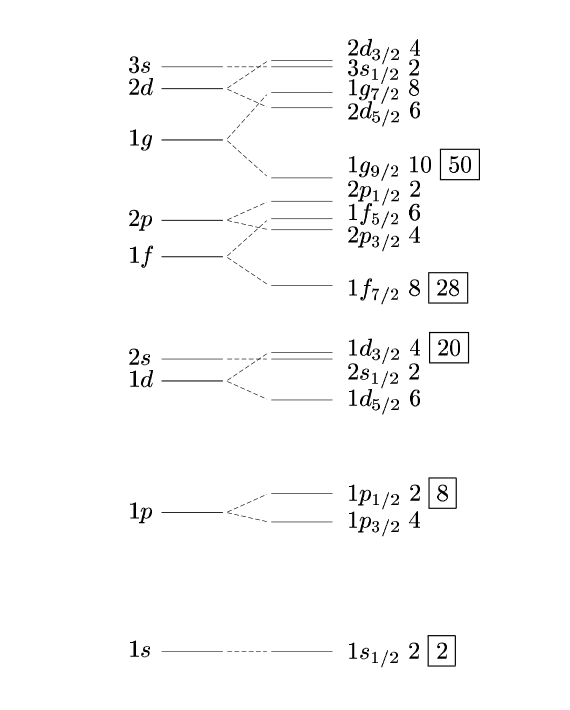
\includegraphics[width=0.6\textwidth]{img/schalen}
	\caption{Energieniveaus des Schalenmodells. Die Spin-Bahn-Kopplung ist hier explizit berücksichtigt. \cite{schalen}}
	\label{schalen}
\end{figure}

\subsection{Emission von $\gamma$-Strahlung}

Nach $\alpha$- und $\beta$-Zerfällen liegen die die Kerne oft in einem angeregten Zustand vor. Die \glqq Abregung\grqq\ geschieht meist über die Aussendung von $\gamma$-Quanten, also hoch-energetischen Photonen. Im Gegensatz zu den elektromagnetischen Übergängen in der Atomhülle, wo fast nur Dipolstrahlung auftritt, sind bei den Übergängen im Kern höhere Multipole (Quadrupol, Oktupol, ...) nicht zu vernachlässigen. 

Statt der Emission von Photonen kann die Energie auch an ein Elektron in der Hülle des Atoms abgegeben werden, welches dadurch aus dem Atom herausgeschlagen wird (Konversionselektronen). Im Gegensatz zur $\beta$-Strahlung entstammen diese jedoch nicht dem Kern selbst und besitzen außerdem ein diskretes Energiespektrum. Bei sehr hohen Energien ist zudem die Bildung und Emission eines Elektron-Positron-Paares im Kern möglich (Paarkonversion).

\subsubsection{Auswahlregeln und Multipolstrahlung}

Bei elektromagnetischen Übergängen muss der Gesamtdrehimpuls erhalten bleiben. Besitzt das emittierte Photon den Drehimpuls $l$ und die beteiligten Kernniveaus die Drehimpulse $I_i$ und $I_f$, dann muss gelten:
\begin{align}
	\left| I_i - I_f\right| \leq l \leq I_i + I_f
\end{align}
Man unterscheidet nun zwischen elektrischer (E$l$) und magnetischer (M$l$) $2^l$-Strahlung (Bsp. $l=1\Longrightarrow$ Dipolstrahlung, $l=2\Longrightarrow$ Quadrupolstrahlung, ...). Mit steigendem $l$ nimmt die Wahrscheinlichkeit für einen solchen Übergang exponentiell ab.

Es lässt sich nun zusätzlich die Paritätsquantenzahl $P=\pm 1$ definieren, welche das Symmetrieverhalten einer Wellenfunktion unter einer Koordinatentransformation $\vec{x}\longrightarrow -\vec{x}$ beschreibt. Es gilt für die Parität von Anfangs- und Endzustand ($P_i$ und $P_f$):
\begin{align}
	\Delta P= P_i\cdot P_f = \begin{cases}
	\left( -1\right)^l\,\,\,\,\,&\text{für E$l$-Strahlung} \\
	\left( -1\right)^{l+1}\,\,\,\,\,&\text{für M$l$-Strahlung}
	\end{cases}
\end{align}

\subsubsection{Winkelverteilung bei $\gamma$-$\gamma$-Kaskaden}

Ausgangspunkt zur Berechnung der theoretisch erwarteten Winkelverteilung ist die Überlegung, dass der Detektor im Vergleich zur Ausdehnung der Quelle sehr weit von dieser entfernt ist (Details im Versuchsaufbau). Das hier nur klassisch betrachtete elektromagnetische Feld kann daher näherungsweise als quellfrei angenommen werden. Die Maxwell-Gleichungen vereinfachen sich daher zu:
\begin{align}
	\begin{split}
		\vec{\nabla}\times\vec{E}=-\frac{\partial B}{\partial t}\qquad\qquad \vec{\nabla}\times\vec{B}=\frac{1}{c^2}\frac{\partial E}{\partial t}\\\vspace{0,2cm}
		\vec{\nabla}\cdot\vec{E}=0 \,\,\qquad\qquad\qquad\vec{\nabla}\cdot\vec{B}=0\qquad\;
	\end{split}
\end{align}
Die Lösungen sind gegeben durch:
\begin{align}
	\begin{split}
		\vec{B}^m_l= f_l(kr)\cdot\vec{L}\cdot Y^m_l(\Theta,\Phi)\qquad ; \qquad \vec{E}^m_l = i \frac{c}{k} \cdot\vec{\nabla}\times \vec{B}^m_l\qquad\text{für $E$-Felder}\\
		\vec{E}^m_l= f_l(kr)\cdot\vec{L}\cdot Y^m_l(\Theta,\Phi)\qquad ; \qquad \vec{B}^m_l = -i \frac{c}{k} \cdot\vec{\nabla}\times \vec{E}^m_l\qquad\text{für $M$-Felder}
	\end{split}
\end{align}
Die Ausstrahlungscharakteristik ist durch den Poynting-Vektor $\vec{S}=\frac{1}{\mu_0}\left( \vec{E}\times\vec{B}\right) $ gegeben. Im Fernfeld gilt:
\begin{align}
	\epsilon_0\left| \vec{E}\right| ^2=\frac{1}{\mu_0}\left| \vec{B}\right| ^2
\end{align}
Damit folgt für die Winkelverteilung insgesamt:
\begin{align}
\begin{split}
\left|\vec{S} \right| \sim \left| \vec{E}\right|^2 \sim \left| \vec{L}\cdot Y^m_l\right|^2\qquad\text{für $E$-Felder}\\
\left|\vec{S} \right| \sim \left| \vec{B}\right|^2 \sim \left| \vec{L}\cdot Y^m_l\right|^2\qquad\text{für $M$-Felder}
\end{split}
\end{align}
Das heißt, über die Kugelflächenfunktionen $Y^m_l(\Theta,\Phi)$ lässt sich die Winkelverteilung berechnen. Für die hier untersuchten $\gamma$-Kaskade beim Zerfall von $^{60}_{27}$Co in $^{60}_{28}$Ni erwartet man:
\begin{align}
	W(\Theta)\sim 1+\frac{1}{8}\cos^2(\Theta)+\frac{1}{24}\cos^4(\Theta)
\end{align}
Damit lässt sich auch die theoretisch erwartete Asymmetrie berechnen:
\begin{align}
	A_\text{theo.}=\frac{W(180\text{°})-W(90\text{°})}{W(90\text{°})}
\end{align}
Aus der gemessenen Koinzidenzrate bei den jeweiligen Winkeln lässt sich analog die experimentelle Asymmetrie berechnen und mit der theoretischen vergleichen:
\begin{align}
A_\text{exp.}=\frac{C(180\text{°})-C(90\text{°})}{C(90\text{°})}
\end{align}
\subsubsection{Wechselwirkung von Photonen mit Materie}

Ein weiterer wichtiger Punkt ist die Absorption von Photonen in Materie. Es gibt drei verschiedene Prozesse zur Absorption von Photonen, die für unterschiedliche Energiebereiche dominant sind:

\begin{description}
	\item[Photoeffekt:]\hfill
	dominant im eV- bis keV-Bereich
	
	Die gesamte Energie des Photons wird auf ein Elektron in der Hülle der Atome des Absorbermaterials übertragen. Dieses Elektron verlässt das Atom und trägt die bei der Ionisation überbleibende Energie als kinetische Energie davon und kann dadurch weitere Atome ionisieren. Der Wirkungsquerschnitt ist proportional zu $Z^5/E_\gamma^3$ ($Z$: Kernladungszahl des Absorbermaterials, $E_\gamma$: Energie der Photonen).
	
	\item[Comptonstreuung:]\hfill 
	dominant im MeV-Bereich
	
	Das Photon wird an einem quasi freiem Elektron gestreut. Der Energieübertrag ist dabei vom Streuwinkel abhängig. Bei einem Winkel von 0° ist der Energieübertrag null, bei einem Winkel von 180° (Rückstreuung) ist er maximal.
	
	\item[Paarproduktion:]\hfill 
	dominant bei Energien über 10\,MeV
	
	Im elektrischen Feld eines Atomkerns  kann die Energie des Photons dazu genutzt werden, um ein Elektron-Positron-Paar zu erzeugen. Dies kann aber offensichtlich nur dann passieren, wenn die Photonenergie die Summe der Ruhemassen von Elektron und Positron (1022\,keV) übersteigt.
\end{description}

\subsection{Positronium}

Trifft ein bei einem $\beta^+$-Zerfall emittiertes Positron auf Materie, so gibt es zunächst durch Stöße mit den enthaltenen Elektronen Energie ab. Ist die Energie des Positrons so weit verringert, dass es thermalisiert ist, kann es entweder mit einem der Elektronen des Materials sofort annihilieren, oder Elektron und Positron gehen in einen gebundenen Zustand, dem Positronium über. Man unterscheidet dabei zwei Arten des Positroniums:

\begin{description}
	\item[Parapositronium:]\hfill
	
	Die Spins von Elektron und Positron sind antiparallel ausgerichtet, es handelt sich also um einen Singulett-Zustand. Es zerfällt mit einer Lebensdauer von 125\,ps meist in zwei 511\,keV Photonen, die sich im 180°-Winkel zueinander ausbreiten. Dies ist der für den Versuch relevante Zustand.
	
	\item[Orthopositronium:]\hfill 
	
	Dies ist der Tripltett-Zustand des Positroniums, die Spins von Elektron und Positron sind parallel ausgerichtet. Es zerfällt mit einer Lebensdauer von 140\,ns in mindestens drei Photonen.
	
\end{description}

\subsection{Szintillatoren}

Bei der Detektion von Gamma-Strahlung ist es zumeist notwendig, die Energie der Photonen soweit zu verringern, dass die Wellenlänge nachher im sichtbaren Bereich liegt. Diese Aufgabe erfüllen Szintillatoren. Treffen hoch-energetische Gamma-Quanten auf das Absorbermaterial des Szintillators, so geben sie über den Comptoneffekt Energie an das Material ab. 

Man unterscheidet zwischen anorganischen Szintillatormaterialien, welche eine hohe Wechselwirkungsrate haben, aber auch eine große Ansprechzeit, und organischen (Plastik-)Szintillatoren, welche weniger mit einfallender Strahlung wechselwirken und dafür schneller ansprechen. Entsprechend eignen sich anorganische eher zur Detektion von Gamma-Strahlung und organische eher für massive Teilchen (Alpha-Teilchen, Spaltbruchstücke, ...). 

In dieser Versuchsreihe werden anorganische Szintillatoren verwendet. Diese besitzen eine Kristallstruktur und können demnach durch das Bändermodell verstanden werden. Gibt ein eintreffendes Photon Energie an eines der Elektronen des Szintillatormaterials ab, so wird dieses in das Leitungsband angehoben, beim Driftprozess kann dieses Elektron dabei weitere Atome ionisieren. 

Entscheidend ist nun, dass bei der Abregung eine geringere Bandlücke überwunden wird als bei der Anregung, sodass die ausgesandten Photonen keine erneute Anregung der Valenzelektronen bewirken können und der Szintillator somit für die Photonen transparent erscheint. Diese Übergänge mit niedriger Energiedifferenz können durch eine geeignete Dotierung erzeugt werden. Die überschüssige Energie wird dabei z.B. durch Gitterschwingungen (Phononen) abgegeben. Die Anzahl der erzeugten Photonen, welche im sichtbaren Wellenlängenbereich liegen, ist proportional zur Energie des einfallenden Gamma-Quants, wodurch diese mithilfe von nachgeschalteten Photomultipliern leicht bestimmt werden kann.


\subsection{Photomultiplier}

Photomultiplier eignen sich zur Detektion einzelner Photonen im sichtbaren Wellenlängenbereich. Damit sie auch ionisierende Strahlung detektieren können, ist ihnen ein Szintillator vorgeschaltet. Die Detektion von Photonen geschieht dabei über den Photoeffekt, bei dem ein eintreffendes Photon ein Elektron aus einer Dynode herauslöst. Da ein einzelnes Elektron nicht als ein ausreichend starker Strom gemessen werden kann, wird mittels einer Beschleunigungsspannung das Elektron auf eine weitere Dynode gelenkt, wo es neue Elektronen herauslösen kann. Dieser Vorgang wird solange wiederholt, bis die Verstärkung groß genug ist, dass ein ausreichender Spannungspuls detektiert werden kann.
	\newpage
	\section{Durchführung}

Bei der Versuchsdurchführung wird zunächst 
	\newpage
	\section{Datenanalyse}

	Dieser Abschnitt umfasst die Auswertung der aufgenommenen Daten.
	Im Folgenden werden die Unsicherheiten sämtlicher Messdaten, Messwerte und Messergebnisse nach GUM\cite{1} bestimmt.
	Für weitere Angaben wird an dieser Stelle auf den Anhang in \cref{sec:anhang} verwiesen.
	Alle konkreten Fit-Parameter finden sich ebenfalls im Anhang in \cref{sec:anhang}.

\subsection{Verzögerungsdauer}
	
	Um möglichst viele Koinzidenzen zu messen, wird die Zählrate nach der Koinzidenzeinheit gegen die eingestellte Verzögerung aufgezeichnet.
	Hierzu wird $^{22}\text{Na}$ verwendet, um durch den Zerfall des Parapositroniums zwei $\gamma$-Quanten im Winkel von \SI{180}{\degree} zu gewährleisten.
	Die Überlagerungswahrscheinlichkeit ist durch eine Gauß-Kurve abgeschätzt und in \cref{fig:zeitdiff} dargestellt.
	Die Verzögerungsdauer ist durch einen analogen Regler mit $\delta t = \SI{2.5}{\nano\second}$ eingestellt worden.
	\begin{figure}[ht]
		\centering
		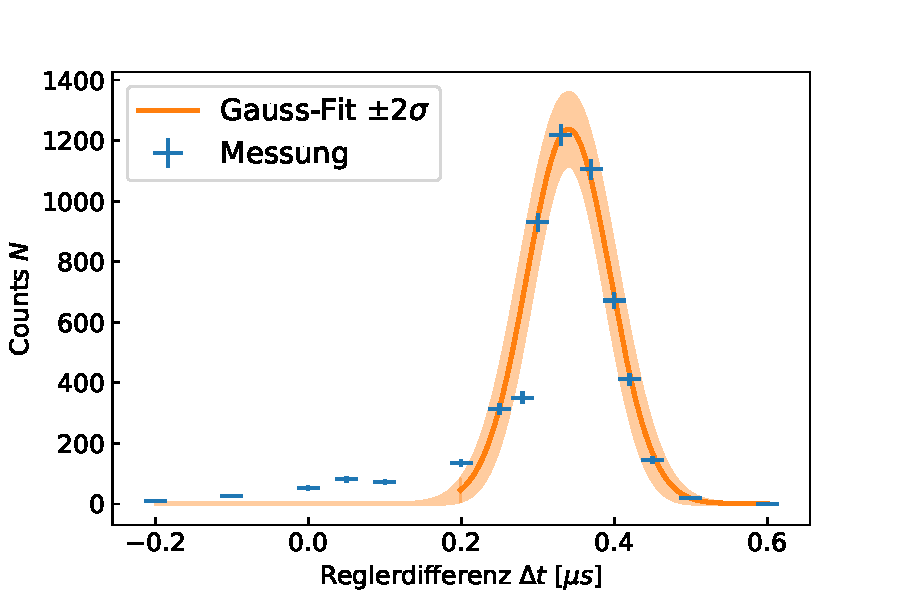
\includegraphics[width=0.7\textwidth]{dat/zeitdifferenz.pdf}
		\caption{Zusammenhang von der eingestellten Verzögerung zwischen beiden Signalen und der Zählrate.
			Die Daten wurden mit einer Gauß-Kurve \\$N(\Delta t) =  A \cdot \exp{-\frac{(\Delta t - \Delta t_0)^2}{2 \sigma_{\Delta t}^2}} + y_0$ angepasst.}
		\label{fig:zeitdiff}
	\end{figure}
	Da Werte mit Verzögerungsdauern kleiner als \SI{0.2}{\micro\second} eine statistisch relevante Abweichung von Null haben, wurden diese nicht in die Anpassung der Gauß-Kurve eingebunden.
	Die Position des Peaks liegt bei $\Delta t_0 = \input{dat/messung1_x0.txt}$.
	In allen folgenden Messungen ist die Signalverzögerung fest auf \SI{333}{\nano\second} eingestellt.
	Diese Einstellung ist mit der Peakposition kompatibel und liefert eine Signaleffizienz von $\epsilon = \input{dat/messung1_eff.txt}$ im Bezug zum Peakmaximum.
	Die Breite $\sigma_{\Delta t} = \input{dat/messung1_d.txt}$ der Kurve ist eine grobe Abschätzung für die Zeitauflösung.
	
\subsection{Koinzidenzauflösungszeit}
	
	Eine genauere Bestimmung der Auflösungszeit $2\theta$ von zwei aufeinander folgenden Signalen ist mit
	\begin{equation}
		N_\text{Z} = N_1 \cdot N_2 \cdot 2\tau \quad \Leftrightarrow \quad  2\tau = \frac{N_Z}{N_1 N_2} = \input{dat/messung2_zweiT.txt}
	\end{equation}
	möglich.
	Dabei sind $N_1 = \input{dat/messung2_det1.txt}$, $N_2 = \input{dat/messung2_det2.txt}$ die Zählraten beider Detektoren vor und $N_Z = \input{dat/messung2_koinz.txt}$ die Zählrate nach der Koinzidenzeinheit.
	Das berechnete Ergebnis liegt in der Größenordnung der Abschätzung.
	Die Quelle hatte im Jahr 1962 eine Aktivität von \SI{3.7}{\mega\becquerel} und somit werden bei der Messung ca. \SI{0.4}{\%} aller Zerfälle gemessen.

	Die Koinzidenzeinheit sieht zwei Signale mit einer absoluten Verzögerung von $\tau$ als Koinzidenz an.
	Somit kann ein Signal relativ zum anderen um maximal $2 \tau$ verschoben werden, ohne aus diesem Interval zu fallen.
	
	Bei dieser Messung wurde $^{137}\text{Cs}$ verwendet, damit ausschließlich einzelne und somit zufällige Koinzidenzen auftreten können.
	
	Durch verschiedene Reflexions- und Streueffekte treten unter bestimmten Winkeln erhöhte Zählraten auf.
	Zum einen werden Photonen bevorzugt bei $\theta = \SI{180}{\degree}$ zurückgestrahlt.
	Zusätzlich werden Photonen durch den Comptoneffekt in der Bleiabschirmung abgelenkt und können bei kleineren Winkeln $\theta$ leicht in den anderen Detektor treffen.
	Bei $\theta = \SI{120}{\degree}$ sind beide Effekte klein und es werden größtenteils die ursprünglichen zufälligen Koinzidenzen der Quelle gemessen.
	Für eine genauere Analyse ist eine tiefere Betrachtung der auftretenden Effekte und der genauen Geometrie des Versuchs erforderlich.
		
\subsection{Vernichtungsstrahung}

	Die $^{22}\text{Na}$-Quelle führt hauptsächlich zur Bildung von Parapositronium, welches dann unter einem Winkel von \SI{180}{\degree} in zwei $\gamma$-Quanten zerfällt.
	In \cref{fig:vernichtung} ist die Zählrate der Koinzidenzen gegen den Winkel $\theta$ dargestellt.
	Dabei wurde die Zählrate an zufälligen Koinzidenzen $N_\text{Z} = \input{dat/messung3_koinz.txt}$ bereits von der gemessenen Zählrate abgezogen, auch wenn sie keinen messbaren Anteil an der Gesamtzählrate hat.
	Theoretisch wird ein scharfer Peak bei genau \SI{180}{\degree} erwartet.
	
	\begin{figure}[ht]
		\centering
		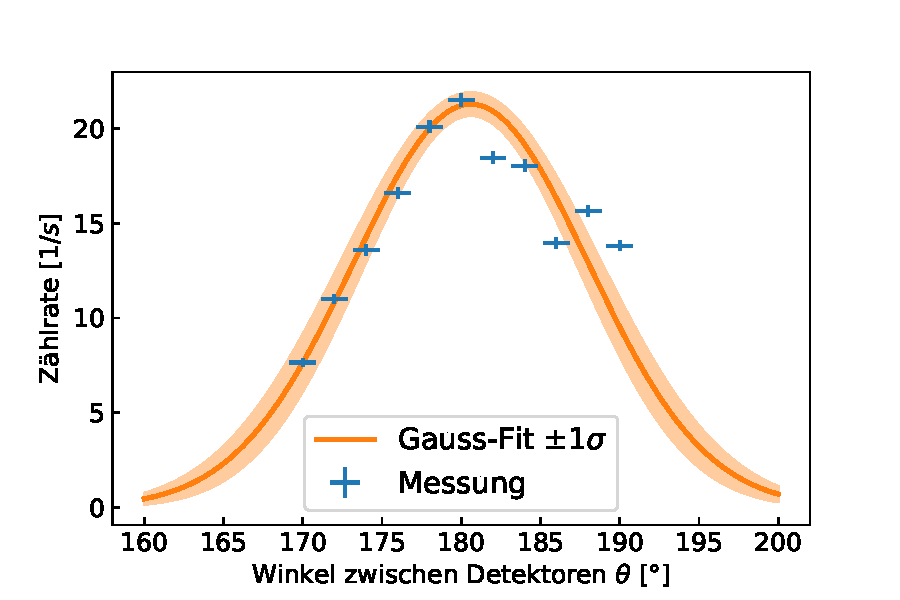
\includegraphics[width=0.7\textwidth]{dat/vernichtung.pdf}
		\caption{Winkelspezifische Zählrate der $^{22}\text{Na}$-Quelle.
			An die Daten wurde eine Gauß-Kurve mit $C(\theta) = A \cdot \exp{-\frac{(\theta - \theta_0)^2}{2 \sigma_{\theta_0}^2}} + y_0$ angepasst.
			Der Peak bei $\theta_0 = \SI{180,6 \pm 0,5}{\degree}$ weißt durch die ausgedehnte Detektorgeometrie eine Breite von $\sigma_{\theta_0} = \SI{7,4 \pm 0,6}{\degree}$ auf.}
		\label{fig:vernichtung}
	\end{figure}

	Wie in der Grafik zu sehen, wird eine gaußförmige Verteilung mit $\theta_0 = \input{dat/messung3_x0.txt}$ und $\sigma_{\theta_0} = \input{dat/messung3_d.txt}$ an die Daten angelegt.
	Daraus ist abzuleiten, dass die Detektorgeometrie einen hohen Einfluss auf die Unsicherheit der betrachteten Winkelmessung hat.
	Im Folgenden ist die Unsicherheit einer Winkelmessung durch $\sigma_{\theta_0}$ gegeben.
	Das $\theta_0$ leicht von \SI{180}{\degree} verschoben ist, kann an einer Schieflage der Quelle während der Messung liegen.
	Da $\theta_0$ allerdings immer noch ausreichend nahe am theoretischen Wert liegt, wurde hier keine weitere Korrektur berechnet.
	
	%TODO fragen beantworten
	
	%TODO mit anteil aus sec2 übereinstimmend?
	%Falls alle Strahlung gemessen wird: 100\% abgedeckter Raumwinkel = 4 pi
	%anteil * 4 pi = 2 pi (1-cos(a / 2))

\subsection{Winkelkorrelation}

	Nachdem aus den vorherigen Messungen Korrekturen und Unsicherheiten des Messapparates bestimmt worden sind, soll nun die Winkelkorrelation der $^{60}\text{Co}$-Probe ermittelt werden.
	Dazu wird zunächst die zufällige Koinzidenzrate zum einen mit der obigen $2\tau$ Methode bestimmt und zum anderen direkt gemessen.
	Die errechnete Koinzidenzrate aus den Einzelraten der Detektoren ergibt $N_\text{Z} = \input{dat/messung4_koinz.txt}$, während die gemessene etwa um den Faktor 10 größer ist.
	Da allerdings insgesamt nur 9 Ereignisse registriert worden sind, können damit keine statistischen Aussagen gemacht werden.
	Sie sind im Verhältnis zur gemessenen Zählrate echter Koinzidenzen verschwindend gering und wirken sich dadurch nicht auf das Ergebnis aus.
	In \cref{fig:theoKurve} sind die Messwerte für $\theta = \SI{90}{\degree}$ und $\theta = \SI{180}{\degree}$ sowie die theoretische Winkelkorrelation eingezeichnet.
	
	\begin{figure}[ht]
		\centering
		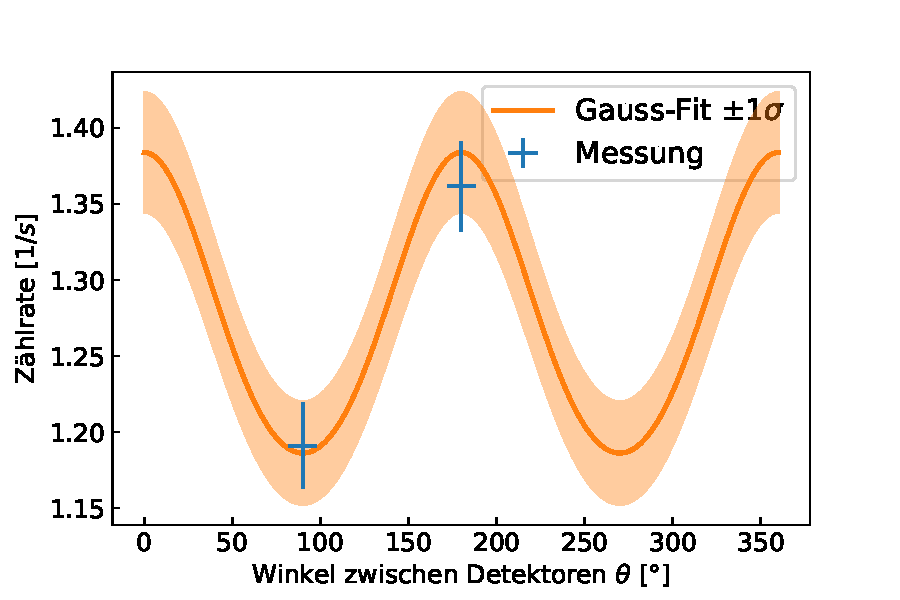
\includegraphics[width=0.7\textwidth]{dat/theoKurve.pdf}
		\caption{Theoretischer Kurvenverlauf und gemessene Einzelwerte.
			Die theoretische Kurve ist proportional zu $1 + \frac{1}{8} \cos^2 \theta + \frac{1}{24} \cos^4 \theta$.}
		\label{fig:theoKurve}
	\end{figure}

	Vergleicht man die theoretische mit der experimentellen Asymmetrie
	\begin{align*}
		A_\text{theo} =&\, \frac{W(\SI{180}{\degree}) - W(\SI{90}{\degree})}{W(\SI{90}{\degree})} = \input{dat/messung4_Atheo.txt} \\
		A_\text{exp} =&\, \frac{C(\SI{180}{\degree}) - C(\SI{90}{\degree})}{C(\SI{90}{\degree})} = \input{dat/messung4_Aexp.txt},
	\end{align*}
	wobei die theoretische Winkelkorrelation $W(\theta)$ aus \cref{eq:korrelation} stammt und $C(\theta)$ die gemessene Zählrate angibt.
	Die gemessene stimmt mit der theoretischen Asymmetrie für die \mbox{$\gamma$-$\gamma$-Kaskade} überein.
	Allerdings ist die Unsicherheit der ermittelten Asymmetrie groß und liegt bei über \SI{20}{\percent}.
	Um die Unsicherheit zu verringern, müssen mehr Messpunkte aufgenommen, die Winkelauflösung verbessert und im Allgemeinen längere Messzeiten eingeplant werden.
	
	
	% --- Fazit des gesammten Versuchs einbinden, falls nötig
	%\IfFileExists{tex/19_Fazit.tex}{
	%	\section{Conclusions}

In this section previous results are summed up and discussed in more depth.

The mean lifetime measurement gives a theory-matching result up to the second decimal place.
Here, the measured lifetime is a lot less than the theoretical value for free muons.
It is also out-of-range of the calculated standard deviation.
As already discussed in the theory section, this could be explained by the capturing processes of negatively charged muons which lower the total mean lifetime of muons.
However, this cannot be verified with the measurements made in this experiment.
Further measurement data needs to be taken.

By simply looking at the data for the characteristics of the detected energy loss spectra of muons at different zenith angles (table \ref{LandauFitParameters}), one can verify two theoretically predicted statements: For larger angles the amplitude of the spectra decreases, while the position of the maximum increases. 

The amplitudes generally match a $\cos^2 (\theta)$-distribution, too.
Nevertheless, four data points are far too few to give a statistical evidence.
Furthermore, the data point at $\theta = 75\,$° matches least the predicted $\cos^2 (\theta)$-distribution which might indicate that it is not proper for large angles.
	 

	%}{}
	
	% --- Anhang einbinden
	\IfFileExists{tex/20_Anhang.tex}{
		\newpage
		\section{Anhang}
		\label{sec:anhang}
		\subsection{Unsicherheiten}\label{VGuD}

Jegliche Unsicherheiten werden nach GUM bestimmt und berechnet.
Die Gleichungen dazu finden sich in \cref{fig:GUM_combine} und \cref{fig:GUM_formula}.
Für die Unsicherheitsrechnungen wurde die Python Bibliothek \texttt{uncertainties} herangezogen, welche den Richtlinien des GUM folgt.

Zur Erstellung von Anpassungskurven wird das Python-Paket \texttt{scipy.odr} verwendet, welches unter anderem die Methoden \texttt{scipy.odr.Model()}, \texttt{scipy.odr.RealData()} und \texttt{scipy.odr.ODR()} zur Verfügung stellt.
Dabei wird auf die sogenannte orthogonale lineare Regression (engl. \emph{Orthogonal Distance Regression} (Abkürzung: ODR)) zurückgegriffen, welche auf der Methode der kleinsten Quadrate basiert und einen modifizierten Levenberg-Marquardt-Algorithmus darstellt.
Für die Parameter von Anpassungskurven und deren Unsicherheiten werden die $x$- und $y$-Unsicherheiten der anzunähernden Werte berücksichtigt und entsprechend gewichtet.
Bei digitalen Messungen wird eine Rechteckverteilung mit $\sigma_X = \frac{\delta X}{2\sqrt{3}}$ und bei analogem Ablesen eine Dreieckverteilung mit $\sigma_X = \frac{\delta X}{2\sqrt{6}}$ angenommen.
Die konkreten Werte der jeweiligen Fehlerintervalle $\delta X$ werden in den entsprechenden Abschnitten angemerkt.

Die jeweiligen $\delta X$ sind im konkreten Abschnitt zu finden.
\begin{figure}[ht]
	\begin{equation*}
		x = \sum_{i=1}^{N} x_i
		;\quad
		\sigma_x = \sqrt{\sum_{i = 1}^{N} \sigma_{x_i}^2}
	\end{equation*}
	\caption{Formel für kombinierte Unsicherheiten des selben Typs nach GUM.}
	\label{fig:GUM_combine}
\end{figure}

\begin{figure}[ht]
	\begin{align*}
		f = f(x_1, \dots , x_N)
		;\quad
		\sigma_f = \sqrt{\sum_{i = 1}^{N}\left(\pdv{f}{x_i} \sigma_{x_i}\right) ^2}
	\end{align*}
	\caption{Formel für sich fortpflanzende Unsicherheiten nach GUM.}
	\label{fig:GUM_formula}
\end{figure}

\subsection{Diagramme}

\begin{figure}[ht]
	\centering
	\begin{subfigure}[c]{0.45\textwidth}		
		\centering	
		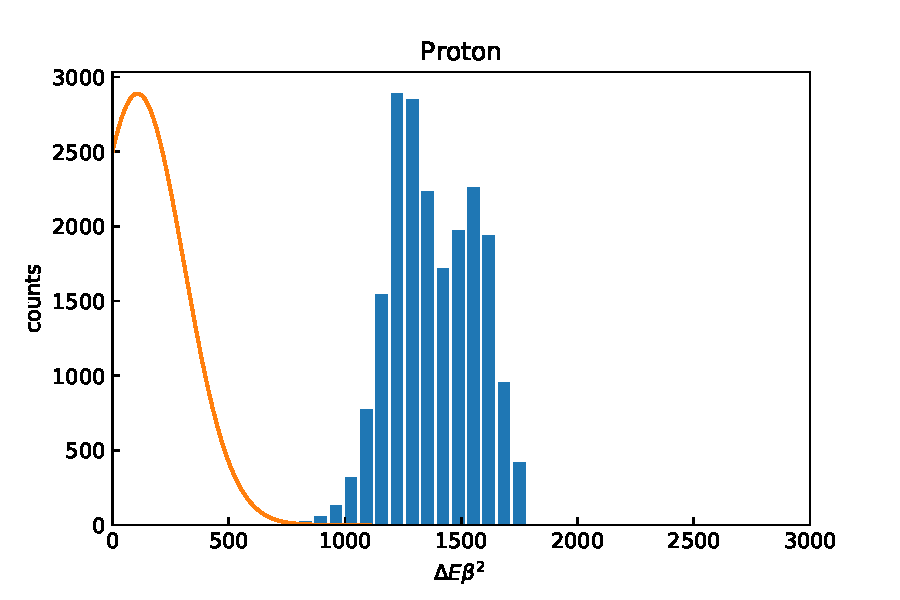
\includegraphics[width=\textwidth]{dat/debeta_Proton.pdf}
	\end{subfigure}
	\begin{subfigure}[c]{0.45\textwidth}
		\centering
		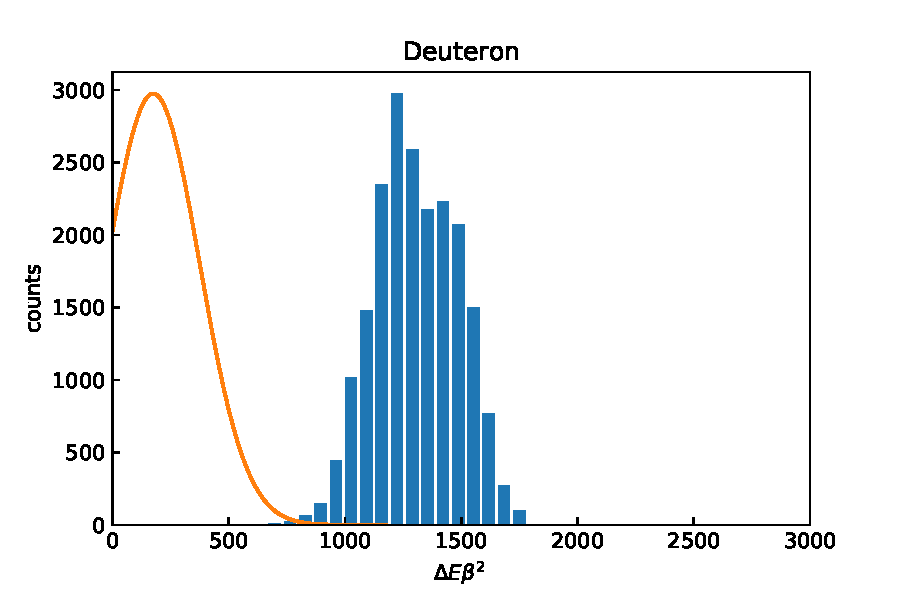
\includegraphics[width=\textwidth]{dat/debeta_Deuteron.pdf}
	\end{subfigure}
	
	\begin{subfigure}[c]{0.45\textwidth}
		\centering
		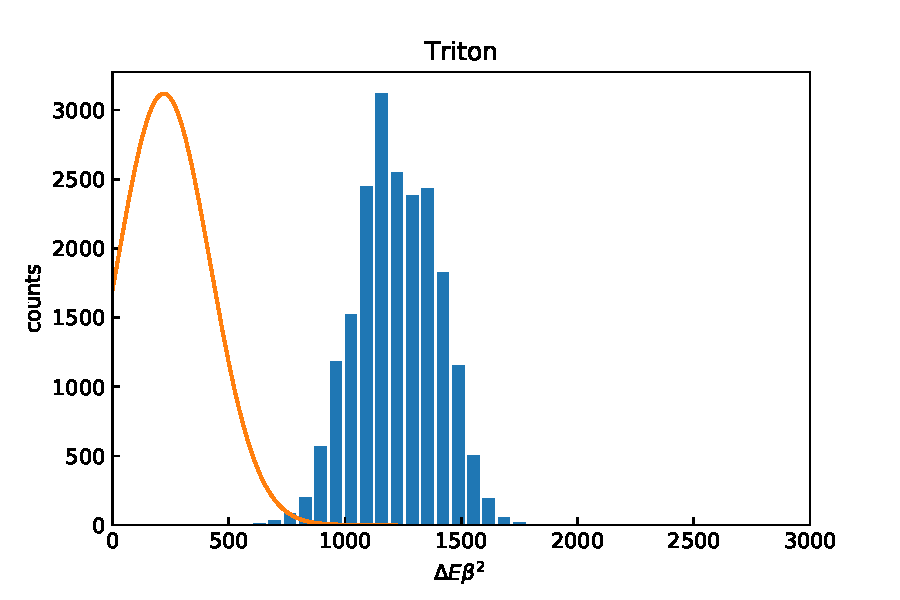
\includegraphics[width=\textwidth]{dat/debeta_Triton.pdf}
	\end{subfigure}
	\begin{subfigure}[c]{0.45\textwidth}
		\centering
		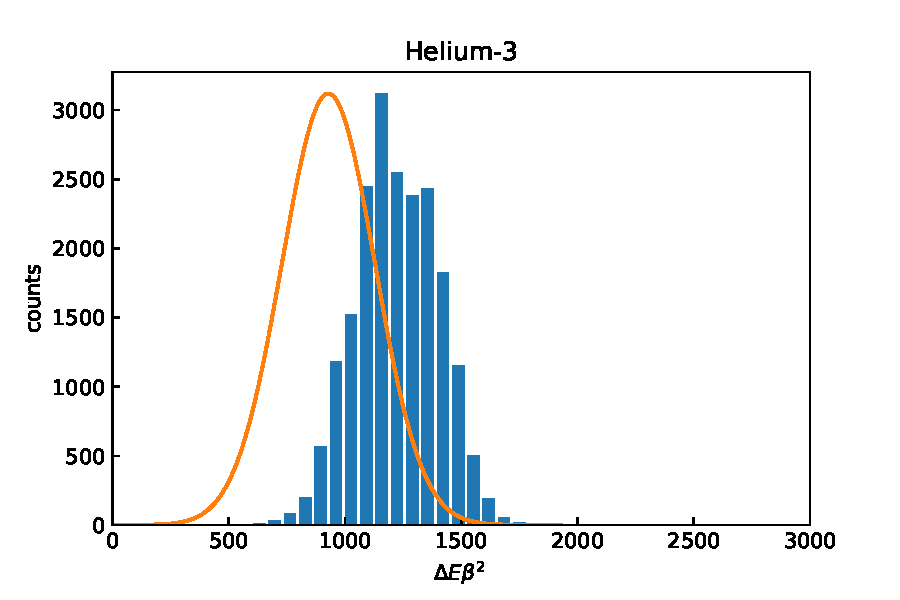
\includegraphics[width=\textwidth]{dat/debeta_Helium-3.pdf}
	\end{subfigure}
	
	\begin{subfigure}[c]{0.45\textwidth}
		\centering
		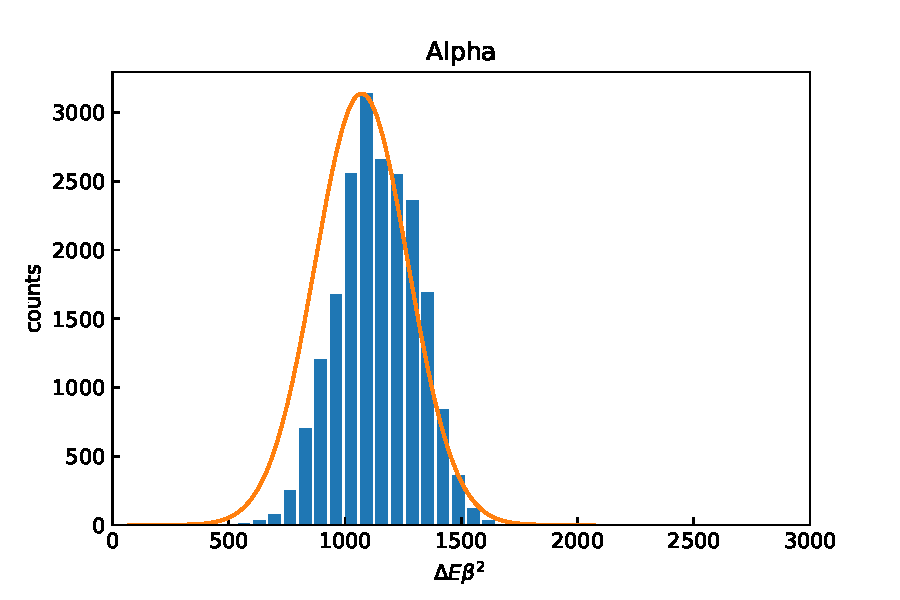
\includegraphics[width=\textwidth]{dat/debeta_Alpha.pdf}
	\end{subfigure}
	\begin{subfigure}[c]{0.45\textwidth}
		\centering
		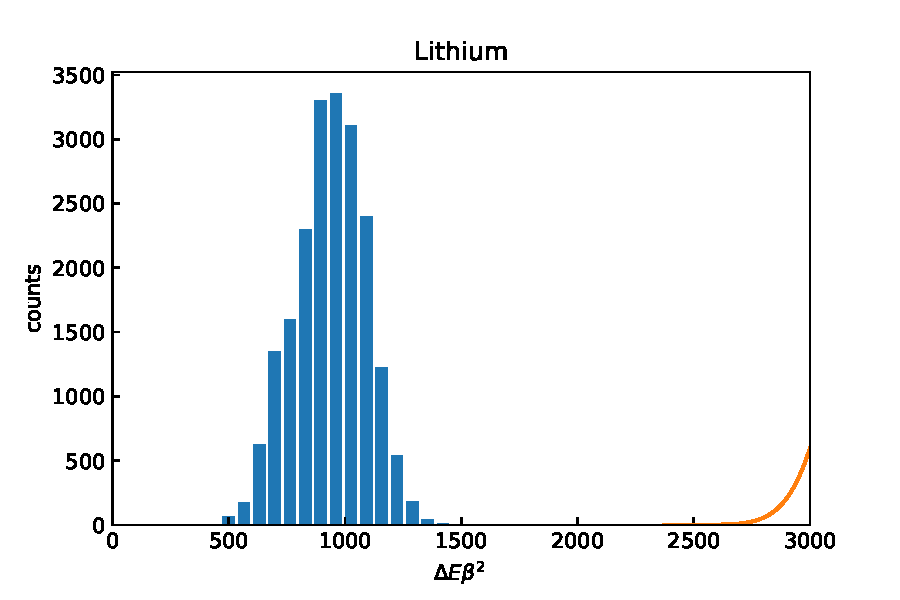
\includegraphics[width=\textwidth]{dat/debeta_Lithium.pdf}
	\end{subfigure}
	
	\caption{$\Delta E \beta^2$ Verteilungen für vermutete Teilchenarten. Eingezeichnet sind die gemessenen Werte, sowie die theoretisch zu erwartenden Verteilungen. $\alpha$-Teilchen geben die Messergebnisse am besten wieder.}
	\label{fig:debeta_full}
\end{figure}

\subsection{Fit-Parameter}
\label{sec:fitval}

\begin{table}[H]
	\centering
	\caption{Fit-Parameter für die normierte Doppelgaussfunktion \mbox{$n(E) = A_1 \cdot \exp{-\frac{(E - E_1)^2}{2 \sigma_1^2}} + A_2 \cdot \exp{-\frac{(E - E_2)^2}{2 \sigma_2^2}} + E_0$} der Dickebestimmung.}
	\label{tab:fitval1}
	\input{dat/m3_fitdaten.txt}
\end{table}
	}{}
	
	\clearpage
	\printbibliography
	
\end{document}
